\chapter*{1. Introducción}\addcontentsline{toc}{chapter}{1. Introducción}\label{cap:intro}

Los videojuegos, pese a su popularidad, presentan muchas incógnitas para alguien que desee iniciarse en su creación, 
pudiendo surgir preguntas tales como:
\begin{itemize}
    \item ¿Cómo organizar el desarrollo de un juego?
    \item ¿Debería crear mi propio motor de juegos?
    \item ¿Qué tecnologías usar?
    \item ¿Qué librerías usar?
\end{itemize}
En los últimos años, gracias a la popularización de motores como Unity\cite{unity}, Unreal\cite{unreal} o
Game Maker\cite{gamemaker} y sus modelos de negocio, que muchas veces permiten el uso del motor sin licencia, mientras el uso
del mismo no sea comercial\cite{unity-pricing}\cite{unreal-pricing}\cite{gamemaker-pricing}, han fomentado el llamado fenómeno \textit{indie} en el que individuos o pequeños grupos de
amigos se juntan para crear un videojuego. Esto junto a la gran cantidad de tutoriales, vídeos y cursos online
ha facilitado mucho esta posibilidad. Como se puede ver en la siguiente \figurename~\ref{engine_distribution}, el uso de estos motores es muy extendido. \footnote{Fuente: \url{https://gamalytic.com/blog/exploring-the-pc-engine-landscape}}

\begin{figure}[h!]
    \centering
    
    \subfloat[Videojuegos indies]{
        \begin{tikzpicture}
        \pie{
            51.9/ Unity,
            27.3/ Otros,
            13.5/ Unreal,
            6.0/ Game Maker,
            1.4/ Godot
        }
        \end{tikzpicture}
        \hspace{2mm}
    }
    \subfloat[Videojuegos AAA]{
        \begin{tikzpicture}
        \pie{
            73.3/ Otros,
            17.7/ Unreal,
            9.0/ Unity
        }
        \end{tikzpicture}
        \hspace{2mm}
    }
    
    \caption{Distribución de motores usados para videojuegos (septiembre de 2023)}
    \label{engine_distribution}
\end{figure}

Pero como se ha demostrado tras la reciente polémica con Unity sobre su nueva monetización retroactiva\cite{unity-polemic},
deberían fomentarse más alternativas y opciones de código abierto para que el ecosistema puede seguir creciendo de una forma
saludable.

Así mismo estos motores muchas veces vienen sobrecargados con funcionalidades que aumentan su complejidad e incrementan
el tiempo para entenderlos o no se ajustan a lo que el usuario necesita. Por suerte la información sobre crear un motor de juegos,
con la expansión de internet, se ha hecho cada vez más accesible, pero muchas veces desperdigada.

Este trabajo se propone por lo tanto crear una fuente única con la que un usuario pueda aprender, sin conocimientos previos
y desde cero, los pasos a realizar para crear un motor de juegos y el contexto de las decisiones tomadas para formar su
propia opinión crítica, así como ofrecer online el fruto de ello con demostraciones para el uso del público general.
De tal forma que los usuarios puedan usar el motor para el desarrollo de sus juegos, si
así lo desean, y encuentren un entorno completo de herramientas listo para ello.

\newpage

\section*{1.1. Motivación y Objetivos}\addcontentsline{toc}{section}{1.1. Motivación y Objetivos}\label{sec:motivation}

La motivación de este proyecto surge a partir de un interés en cómo funcionan por dentro los motores de juegos,
así como con la realización de la falta de información en profundidad que cubra en conjunto todas las parte del proceso
de realizar uno. El proyecto se orienta dentro un marco didáctico y formativo, con el deseo de ofrecer más opciones
gratuitas a las disponibles actualmente. Los objetivos de este proyecto son las siguientes:

\begin{enumerate}[label=\textbf{O\arabic*.}]
    \item Análisis de las soluciones disponibles en el mercado y sus principales diferencias y ventajas en las herramientas que ofrecen.
    \item Estudio de los componentes de un motor de juegos e implementación de forma eficiente.
    \item Desarrollo de un motor de juegos, de código abierto y listo para uso profesional, abstrayendo al usuario toda complejidad a través de una API.
    \item Objetivo didáctico del motor, para ello:
    \begin{enumerate}[label=\textbf{O4.\arabic*.}]
        \item Creación de diagramas y videos tutoriales explicando cada parte del motor de juegos y su uso.
        \item Programación de diferentes casos de uso del motor y una plantilla ejemplo de juego usando el motor.
        \item Elaboración de diagramas y videos tutoriales explicando la creación de un juego de plataforma
         \gls{2d-es} usando el motor y haciendo uso de la plantilla.
    \end{enumerate}
\end{enumerate}

\newpage

\section*{1.2. Metodología}\addcontentsline{toc}{section}{1.2. Metodología}\label{sec:methodology}

Después de un análisis previo de los componentes necesarios para el motor de juegos y demostraciones necesarias,
se organizaron las fases del proyecto usando la herramienta \textit{Trello} \figurename~\ref{trello_tool}, y se establecieron fechas concretas para
cada fase, en reuniones bimensuales utilizando \textit{Google meets}.
\begin{figure}[h!]
    \centering
    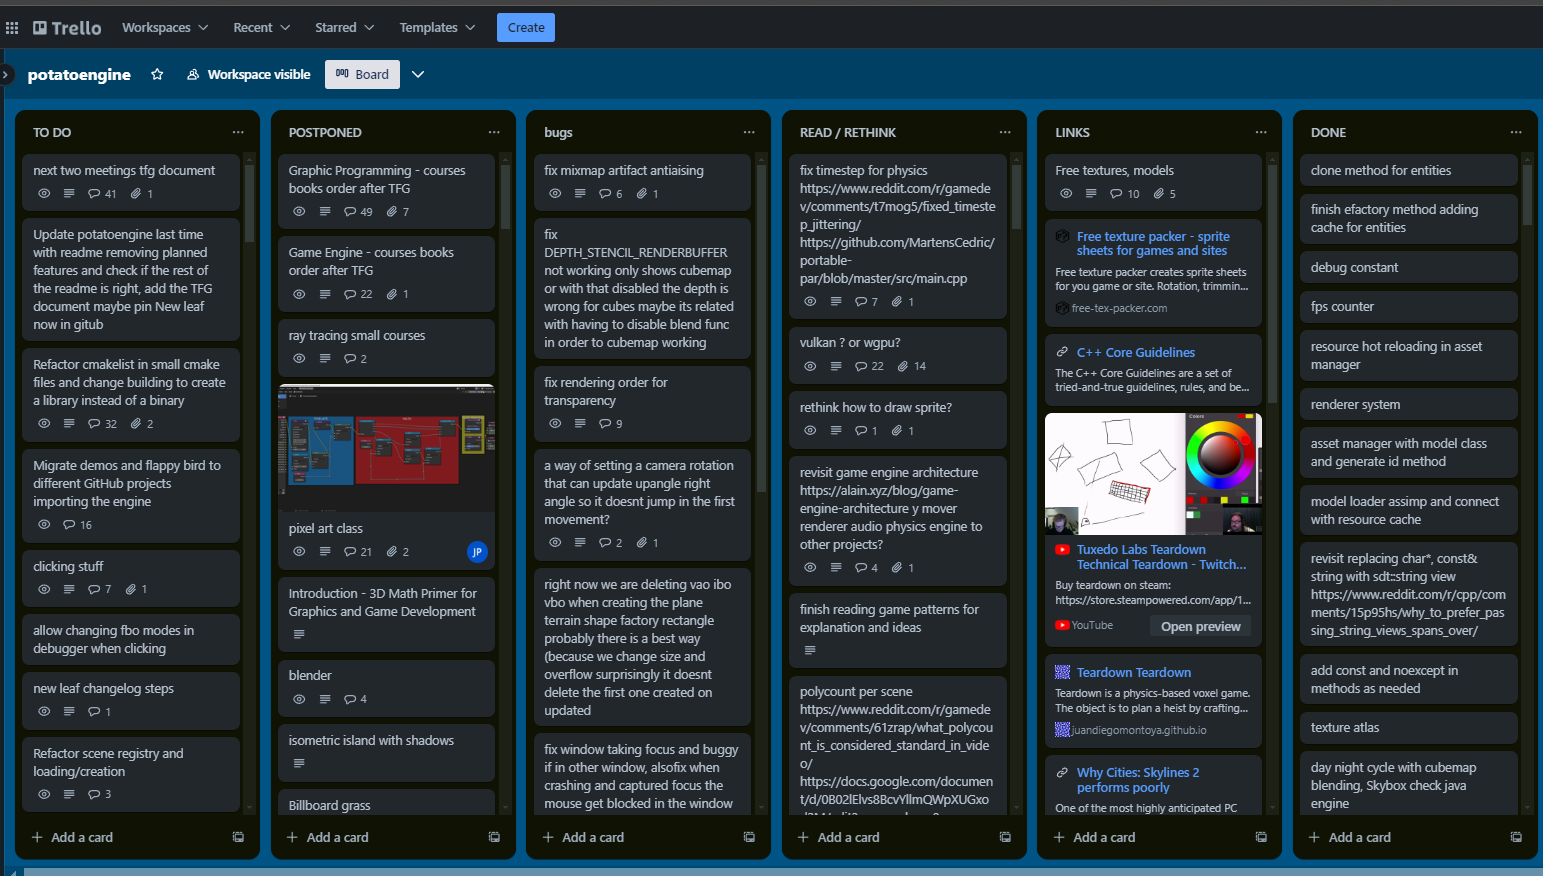
\includegraphics[scale=0.40]{trello}
    \caption{Organización de fases y tareas con Trello}
    \label{trello_tool}
\end{figure}

Las fases del proyecto se han enfocado usando la metodología de Prototipo, permitiendo una iteración rápida
sobre el feedback dado por el coordinador del proyecto y una validación de los objetivos deseados en cada iteración \figurename~\ref{prototype_methodology}.
El proyecto se ha realizado usando \textit{Github} dado que uno de los objetivos era que fuera de código abierto y para
mantener un control de versión. Se puede observar en la \figurename~\ref{github_tool} como el proyecto 
contiene un histórico de todas las versiones o \textit{commits} realizados así como descripciones.

\begin{figure}[h!]
    \centering
    \smartdiagram[circular diagram:clockwise]{Análisis, Diseño, Desarrollo, Validación, Feedback}
    \caption{Metodología de Prototipo}
    \label{prototype_methodology}
\end{figure}

\begin{figure}[h!]
    \centering
    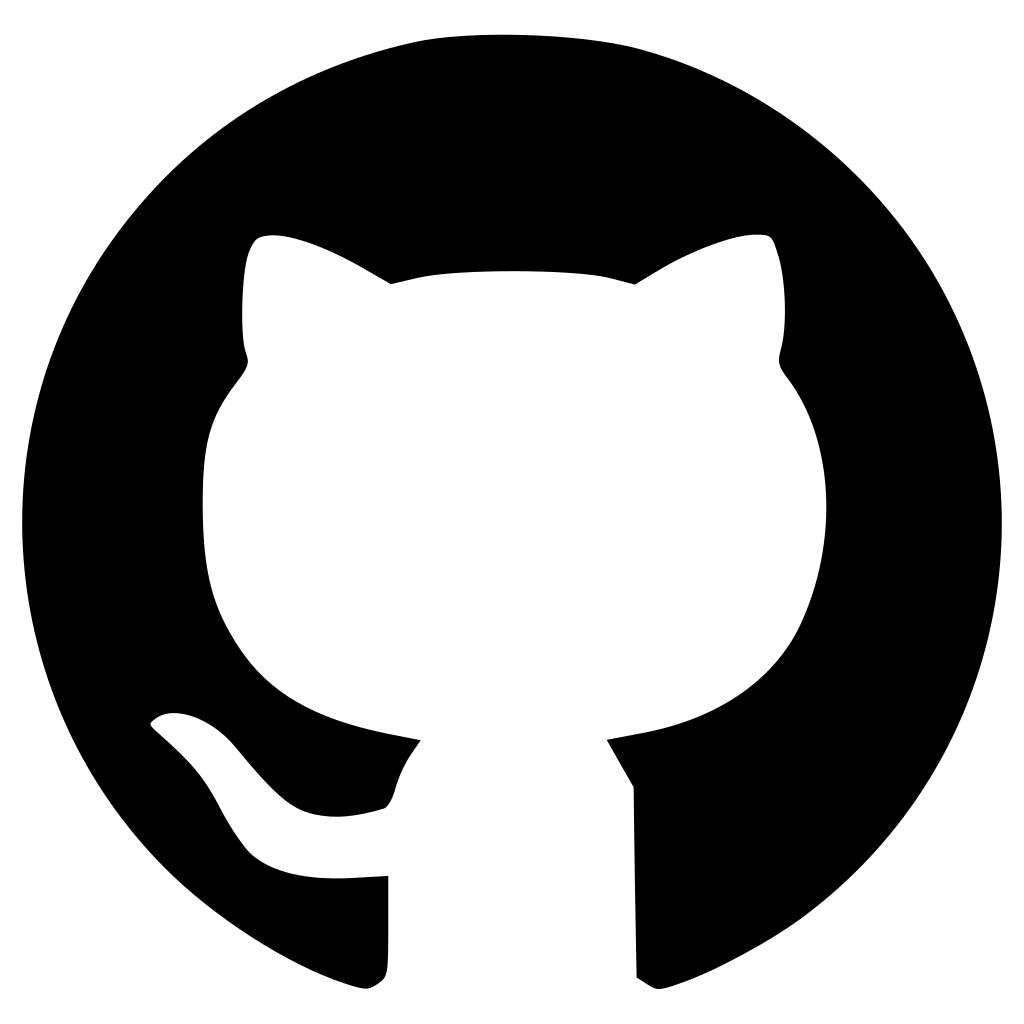
\includegraphics[scale=0.35]{github}
    \caption{Control de versión con Github}
    \label{github_tool}
\end{figure}

\clearpage

\section*{1.3. Estructura de la memoria}\addcontentsline{toc}{section}{1.3. Estructura de la memoria}\label{sec:structure}

La memoria se estructura en una serie de capítulos, en este primero se discute la motivación y objetivos del \gls{tfg},
así como la metodología que se seguirá, el segundo capítulo tratará sobre el análisis, conclusiones de los trabajos
relacionados y tecnologías empleadas / librerías que han ayudado al desarrollo del motor, permitiendo tener una idea clara
de que se necesitará de cara a la fase de diseño del prototipo.

Los siguientes tres capítulos comprenderán el diseño, prototipado y validación del motor, explicando en detalle cada
componente del motor, decisiones tomadas y comparación entre otras posibles soluciones.

Por último se cierra el documento con las conclusiones del proyecto, reflexiones y líneas futuras de mejoras posibles
al motor de juegos. El proyecto se complementa con una lista de acrónimos, bibliografía y un anexo profundizando en partes teóricas.
